\documentclass[9pt,compress,t,aspectratio=169]{beamer}
\usepackage{animate}
\usepackage{graphicx}
\usepackage{setspace}
\usepackage{textcomp}
\usepackage{appendixnumberbeamer}
\usepackage{algorithm}
\usepackage{algorithmic}
\usepackage{caption}
\captionsetup[figure]{labelformat=empty}
\usetheme{RRgroup3}

\usepackage{nth}
\usepackage{amsmath}
\usepackage{stmaryrd}
\usepackage{centernot}
\usepackage{ragged2e}
\usepackage{bm}
\usepackage{moreverb}
\usepackage{tabu}
\usepackage{siunitx}
\usepackage[version=4]{mhchem}
\usepackage[table]{colortbl}
\usepackage[normalem]{ulem}
\usepackage[justification=centering]{caption}
\usepackage{alltt} 
\usepackage{multirow}
\usepackage[mathscr]{euscript}
\usepackage{psfrag}
\usepackage{url}
\usepackage{csquotes}
\usepackage{booktabs}
\usepackage{physics}
\usepackage{xfrac}

%%%%%% Hyperref %%%%%%
\hypersetup{
    pdftitle={},
    pdfauthor={},
    pdfsubject={},
    pdfkeywords=,
    linkcolor=black,
    unicode=false,
    pdftoolbar=true,
    pdfmenubar=true,
    pdffitwindow=true,
    pdfnewwindow=true,
    colorlinks=true,
    citecolor=mitred,
	urlcolor=mitbrightred,
    pdfinfo={UserProperties=yes}
}

%%%%%% Bibliography %%%%%%
\usepackage[
	backend=biber,
	style=authoryear-comp,
	doi=false,
	url=false,
	isbn=false,
	arxiv=false,
	maxbibnames=99,
	hyperref=true,
	sorting=none,
	eprint=false,
	maxcitenames=2,
	uniquelist=false
]{biblatex}

% Use ampersand instead of word "and" in in-text citations
\renewcommand*{\finalnamedelim}{%
  \ifnumgreater{\value{liststop}}{2}{\finalandcomma}{}%
  \addspace\&\space}
\setlength{\bibitemsep}{0.8ex}

% Set height of red region on title frame
% \newcommand{\colorfulTitle}{50}
% \showTim% Show Tim the Beaver on standout frames (commented out - may not be available)

%%% Local Variables:
%%% mode: latex
%%% TeX-master: "presentation"
%%% End:


\usepackage{xcolor}

\definecolor{myblue1}{RGB}{0, 176, 240}
\definecolor{mypurple1}{RGB}{112, 48, 160}
\definecolor{mygreen1}{RGB}{0, 176, 80}
\definecolor{myred1}{rgb}{1.0, 0.0, 0.0}

% Some custom commands
\newcommand{\noIndentItem}{\settowidth{\leftmargini}{\usebeamertemplate{itemize item}}\addtolength{\leftmargini}{\labelsep}}
\newcommand{\jump}[1]{\llbracket #1 \rrbracket}
\newcommand{\avg}[1]{\left\{ #1 \right\}}

% Set presentation options
\setbeamerfont{title}{size=\LARGE}
\setbeamerfont{frametitle}{size=\LARGE}
\setbeamerfont{block body}{size=\footnotesize}
\setbeamerfont{normal text}{size=\footnotesize}
\setbeamerfont{subsection in toc}{size=\small}
\setbeamertemplate{subsection in toc}[subsections numbered]
\setbeamertemplate{subsection in toc}{\leavevmode\leftskip=2em$\bullet$\hskip0.5em\inserttocsubsection\par}
\setbeamertemplate{footline}[author+institution+page]
\newcommand{\colorfulTitle}{}
\setbeamercolor{block title}{bg=black!20,fg=mitred}

\title{Fast methods for PDEs: Final Project}
\subtitle{Spectral HPS scheme for 2D Linear Elasticity}
\author{Giorgos Tsilimidos}
\date{\today}

\addbibresource{bibliography.bib}
\graphicspath{{Figures/}}

%%%%%%%%%%%%%%%%%%%%%%%%%%%%%%% DOCUMENT %%%%%%%%%%%%%%%%%%%%%%%%%%%%%%%%%%%%
\begin{document}
\titleframe{}

\section{Overview}

% ============================================================================
\begin{frame}{Motivation}
\begin{columns}[T]
\begin{column}{0.6\textwidth}
\textbf{2D Linear Elasticity}
\[
\nabla \cdot \boldsymbol{\sigma} + \mathbf{f} = \mathbf{0}, \quad \boldsymbol{\sigma} = 2\mu\boldsymbol{\epsilon} + \lambda(\mathrm{tr}\,\boldsymbol{\epsilon})\mathbf{I}, \quad
\boldsymbol{\epsilon} = \frac{1}{2}(\nabla \mathbf{u} + \nabla \mathbf{u}^T)
\]
Navier-Lame formulation (component form for plane strain):
\[
-(2\mu+\lambda)\frac{\partial^2 u_x}{\partial x^2} - \mu\frac{\partial^2 u_x}{\partial y^2} - (\lambda+\mu)\frac{\partial^2 u_y}{\partial x \partial y} = f_x
\]
\[
-\mu\frac{\partial^2 u_y}{\partial x^2} - (2\mu+\lambda)\frac{\partial^2 u_y}{\partial y^2} - (\lambda+\mu)\frac{\partial^2 u_x}{\partial x \partial y} = f_y
\]

\vspace{0.3cm}
\textbf{Two Benchmarks}
\begin{itemize}
  \item Smooth manufactured solution — spectral convergence?
  \item Mode I crack-tip singularity — algebraic convergence?
\end{itemize}
\end{column}
\begin{column}{0.4\textwidth}
\textbf{Tool: JAX-HPS}
\begin{itemize}
  \item Hierarchical Poincaré-Steklov spectral element solver
  \item Polynomial degree $p$, refinement depth $L$
  \item hp-convergence study: vary $p \in \{3,4,6,8,12,16\}$ and $L \in \{2,3,4\}$
\end{itemize}

\vspace{0.3cm}
\textbf{Acknowledgements}
Based on \texttt{jaxhps} by O.~Meliao — \texttt{github.com/meliao/jaxhps}

\end{column}
\end{columns}
\end{frame}

% ============================================================================
\begin{frame}{Method: Hierarchical Poincaré-Steklov (HPS)}
\begin{columns}[T]

\begin{column}{0.6\textwidth}

\textbf{Key Idea}
Instead of solving one big global system, solve many small spectral problems locally, then 
merge them hierarchically through boundary operators.

\textbf{Two-Pass Solver}
\begin{enumerate}
  \item \textbf{Up-pass}: build Schur complements, leaf $\to$ root
  \item \textbf{Down-pass}: recover solution, root $\to$ leaves
\end{enumerate}

\textbf{ADI (Alternating Direction Implicit)}

\smallskip
Treat coupling term $\mathcal{L}_{xy}=(\lambda+\mu)\partial_{xy}$ as source and iterate:
\[
\mathcal{L}_{xx}\, u_x^{(k+1)} = f_x - \mathcal{L}_{xy}\, u_y^{(k)}
\]
\[
\mathcal{L}_{yy}\, u_y^{(k+1)} = f_y - \mathcal{L}_{xy}\, u_x^{(k+1)}
\]
\begin{itemize}
    \item Each line is a scalar HPS solve with updated RHS.
    \item In some cases (rectangle), this converges in fixed number of iterations independent of discretization.
\end{itemize}

\end{column}

\begin{column}{0.4\textwidth}
\centering
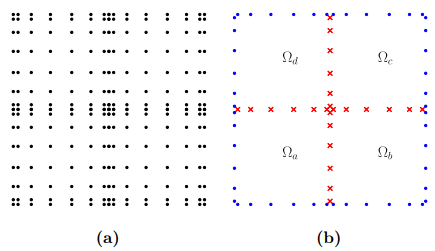
\includegraphics[width=0.75\textwidth]{Figures/chebyshev_grid.png}\\[0.1cm]
\scriptsize Chebyshev grid on a leaf element

\vspace{0.3cm}
\raggedright
\textbf{Discretization}
\begin{itemize}
  \item Quadtree domain: $L$ refinement levels
  \item Leaf $K$: $p\times p$ Chebyshev interior nodes
\end{itemize}
\end{column}

\end{columns}
\end{frame}

\section{Smooth Problem}

% ============================================================================
\begin{frame}{Problem 1: Smooth Manufactured Solution}
\begin{columns}[T]
\begin{column}{0.38\textwidth}
\small
\textbf{Domain:} $\Omega = [-1,1]^2$, $\lambda=\mu=1$

\textbf{Exact solution}
\[
u_x = \sin(\pi x)\sin(\pi y)
\]
\[
u_y = \cos(\pi x)\cos(\pi y)
\]

\textbf{Source term}
\[
f_x = 2\mu\pi^2\sin(\pi x)\sin(\pi y)
\]
\[
f_y = -(\lambda+2\mu)\pi^2\cos(\pi x)\cos(\pi y)
\]

\vspace{0.2cm}
All derivatives analytic $\Rightarrow$ \textbf{exponential convergence}.
\end{column}
\begin{column}{0.65\textwidth}
\centering
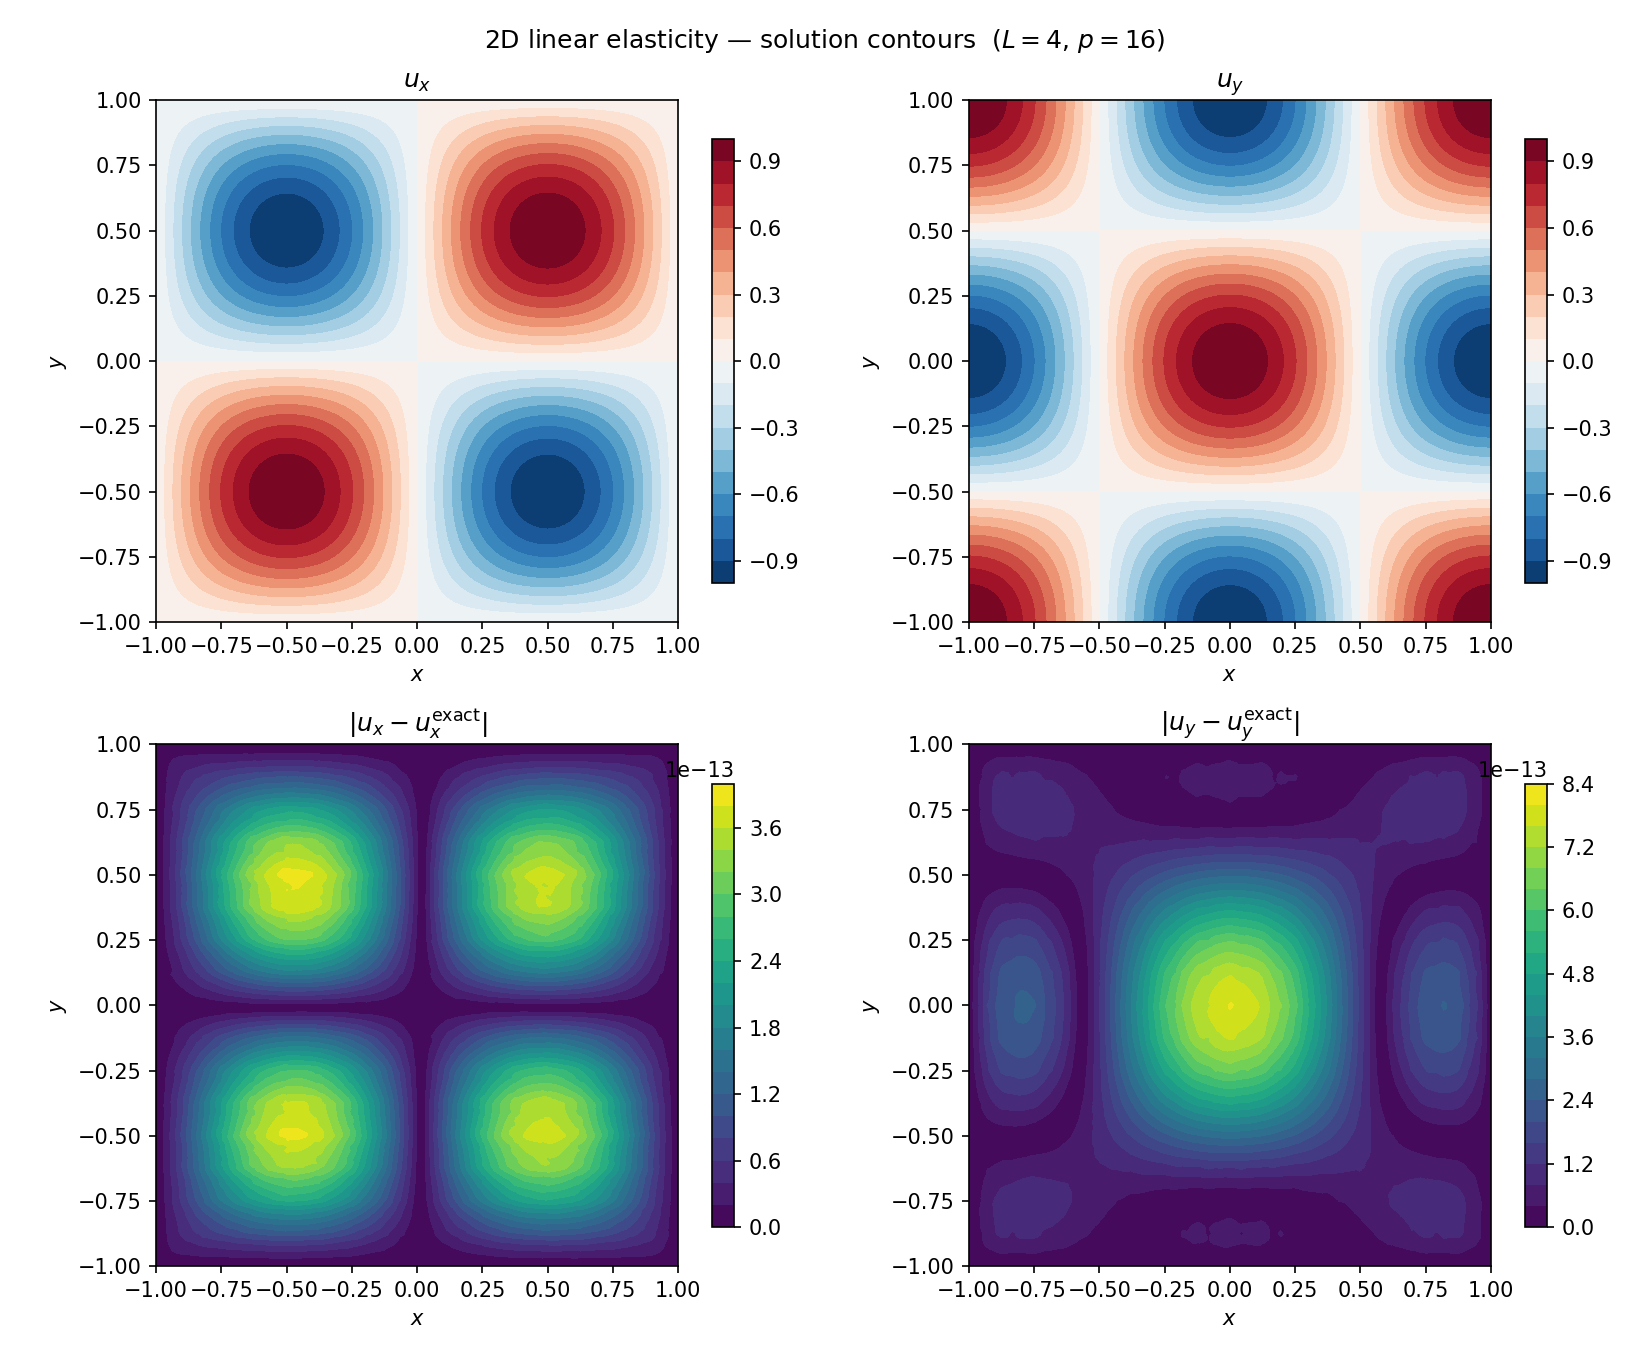
\includegraphics[width=0.9\textwidth]{../data/examples/linear_elasticity_2D/solution_contours.png}
\end{column}
\end{columns}
\end{frame}

% ============================================================================
\begin{frame}{Problem 1: Convergence}
\centering
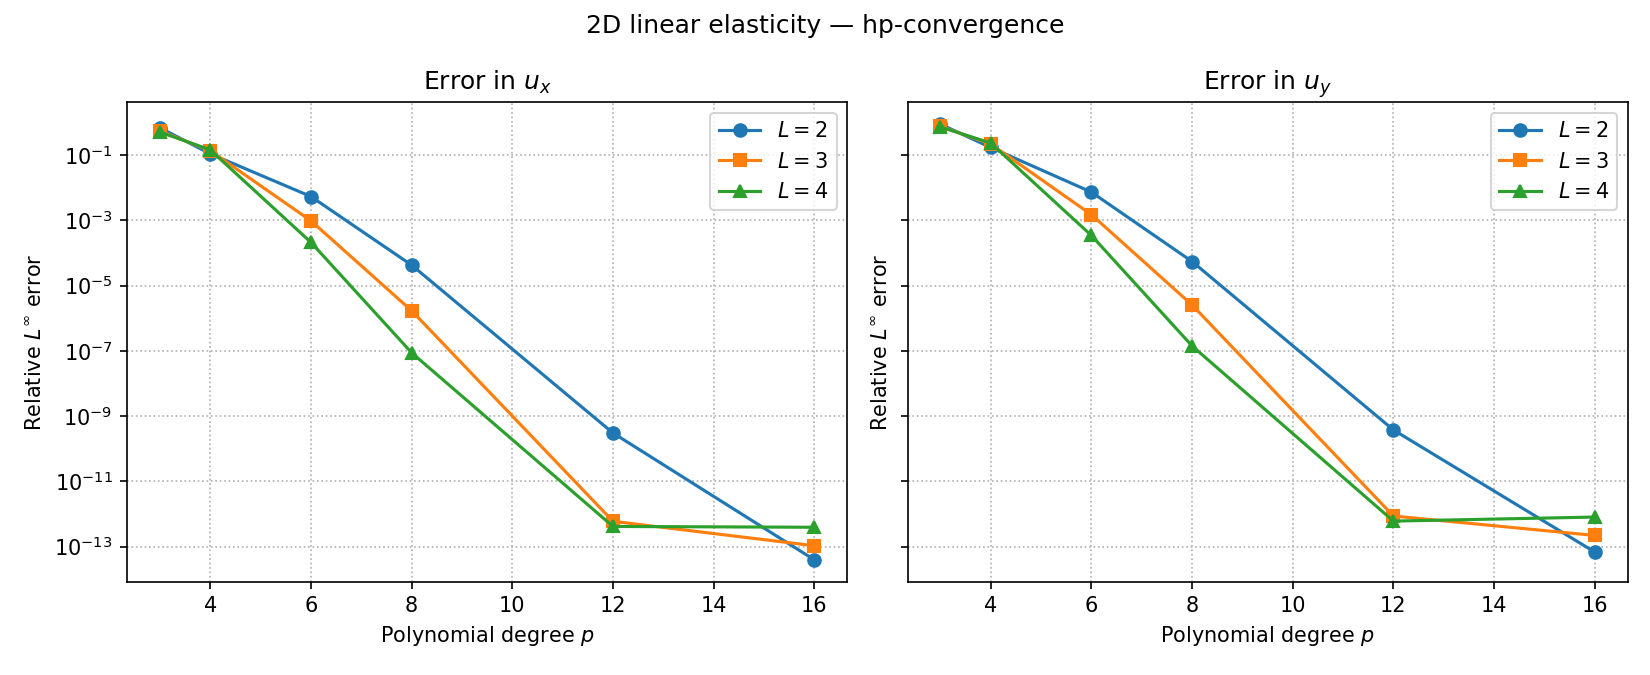
\includegraphics[height=0.82\textheight]{../data/examples/linear_elasticity_2D/error_vs_p.png}
\end{frame}

\section{Singular Problem}

% ============================================================================
\begin{frame}{Problem 2: Mode I Crack-Tip Singularity}
\begin{columns}[T]
\begin{column}{0.4\textwidth}
\small
\textbf{Williams Expansion (Mode I, plane strain)}
\[
u_x = \frac{K_I}{2\mu}\sqrt{\frac{r}{2\pi}}\cos\tfrac{\theta}{2}(\kappa - \cos\theta)
\]
\[
u_y = \frac{K_I}{2\mu}\sqrt{\frac{r}{2\pi}}\sin\tfrac{\theta}{2}(\kappa - \cos\theta)
\]
$\kappa = 3-4\nu$

\vspace{0.2cm}
\textbf{Stress singularity}
\[
\boldsymbol{\sigma}(r,\theta) = \frac{K_I}{\sqrt{2\pi r}}\,\mathbf{f}(\theta) + O(r^{1/2})
\]
$\nabla u \sim r^{-1/2}$ as $r\to 0^+$

\vspace{0.2cm}
Dirichlet BCs from exact solution.
\end{column}
\begin{column}{0.6\textwidth}
\centering
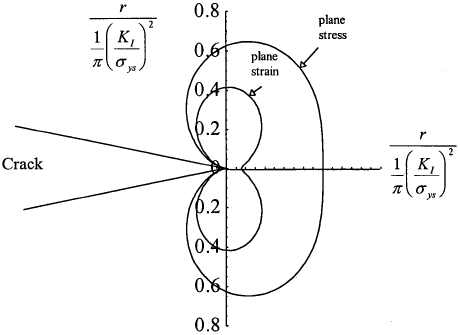
\includegraphics[width=0.5\textwidth]{Figures/crack_tip.png}\\[0.2cm]
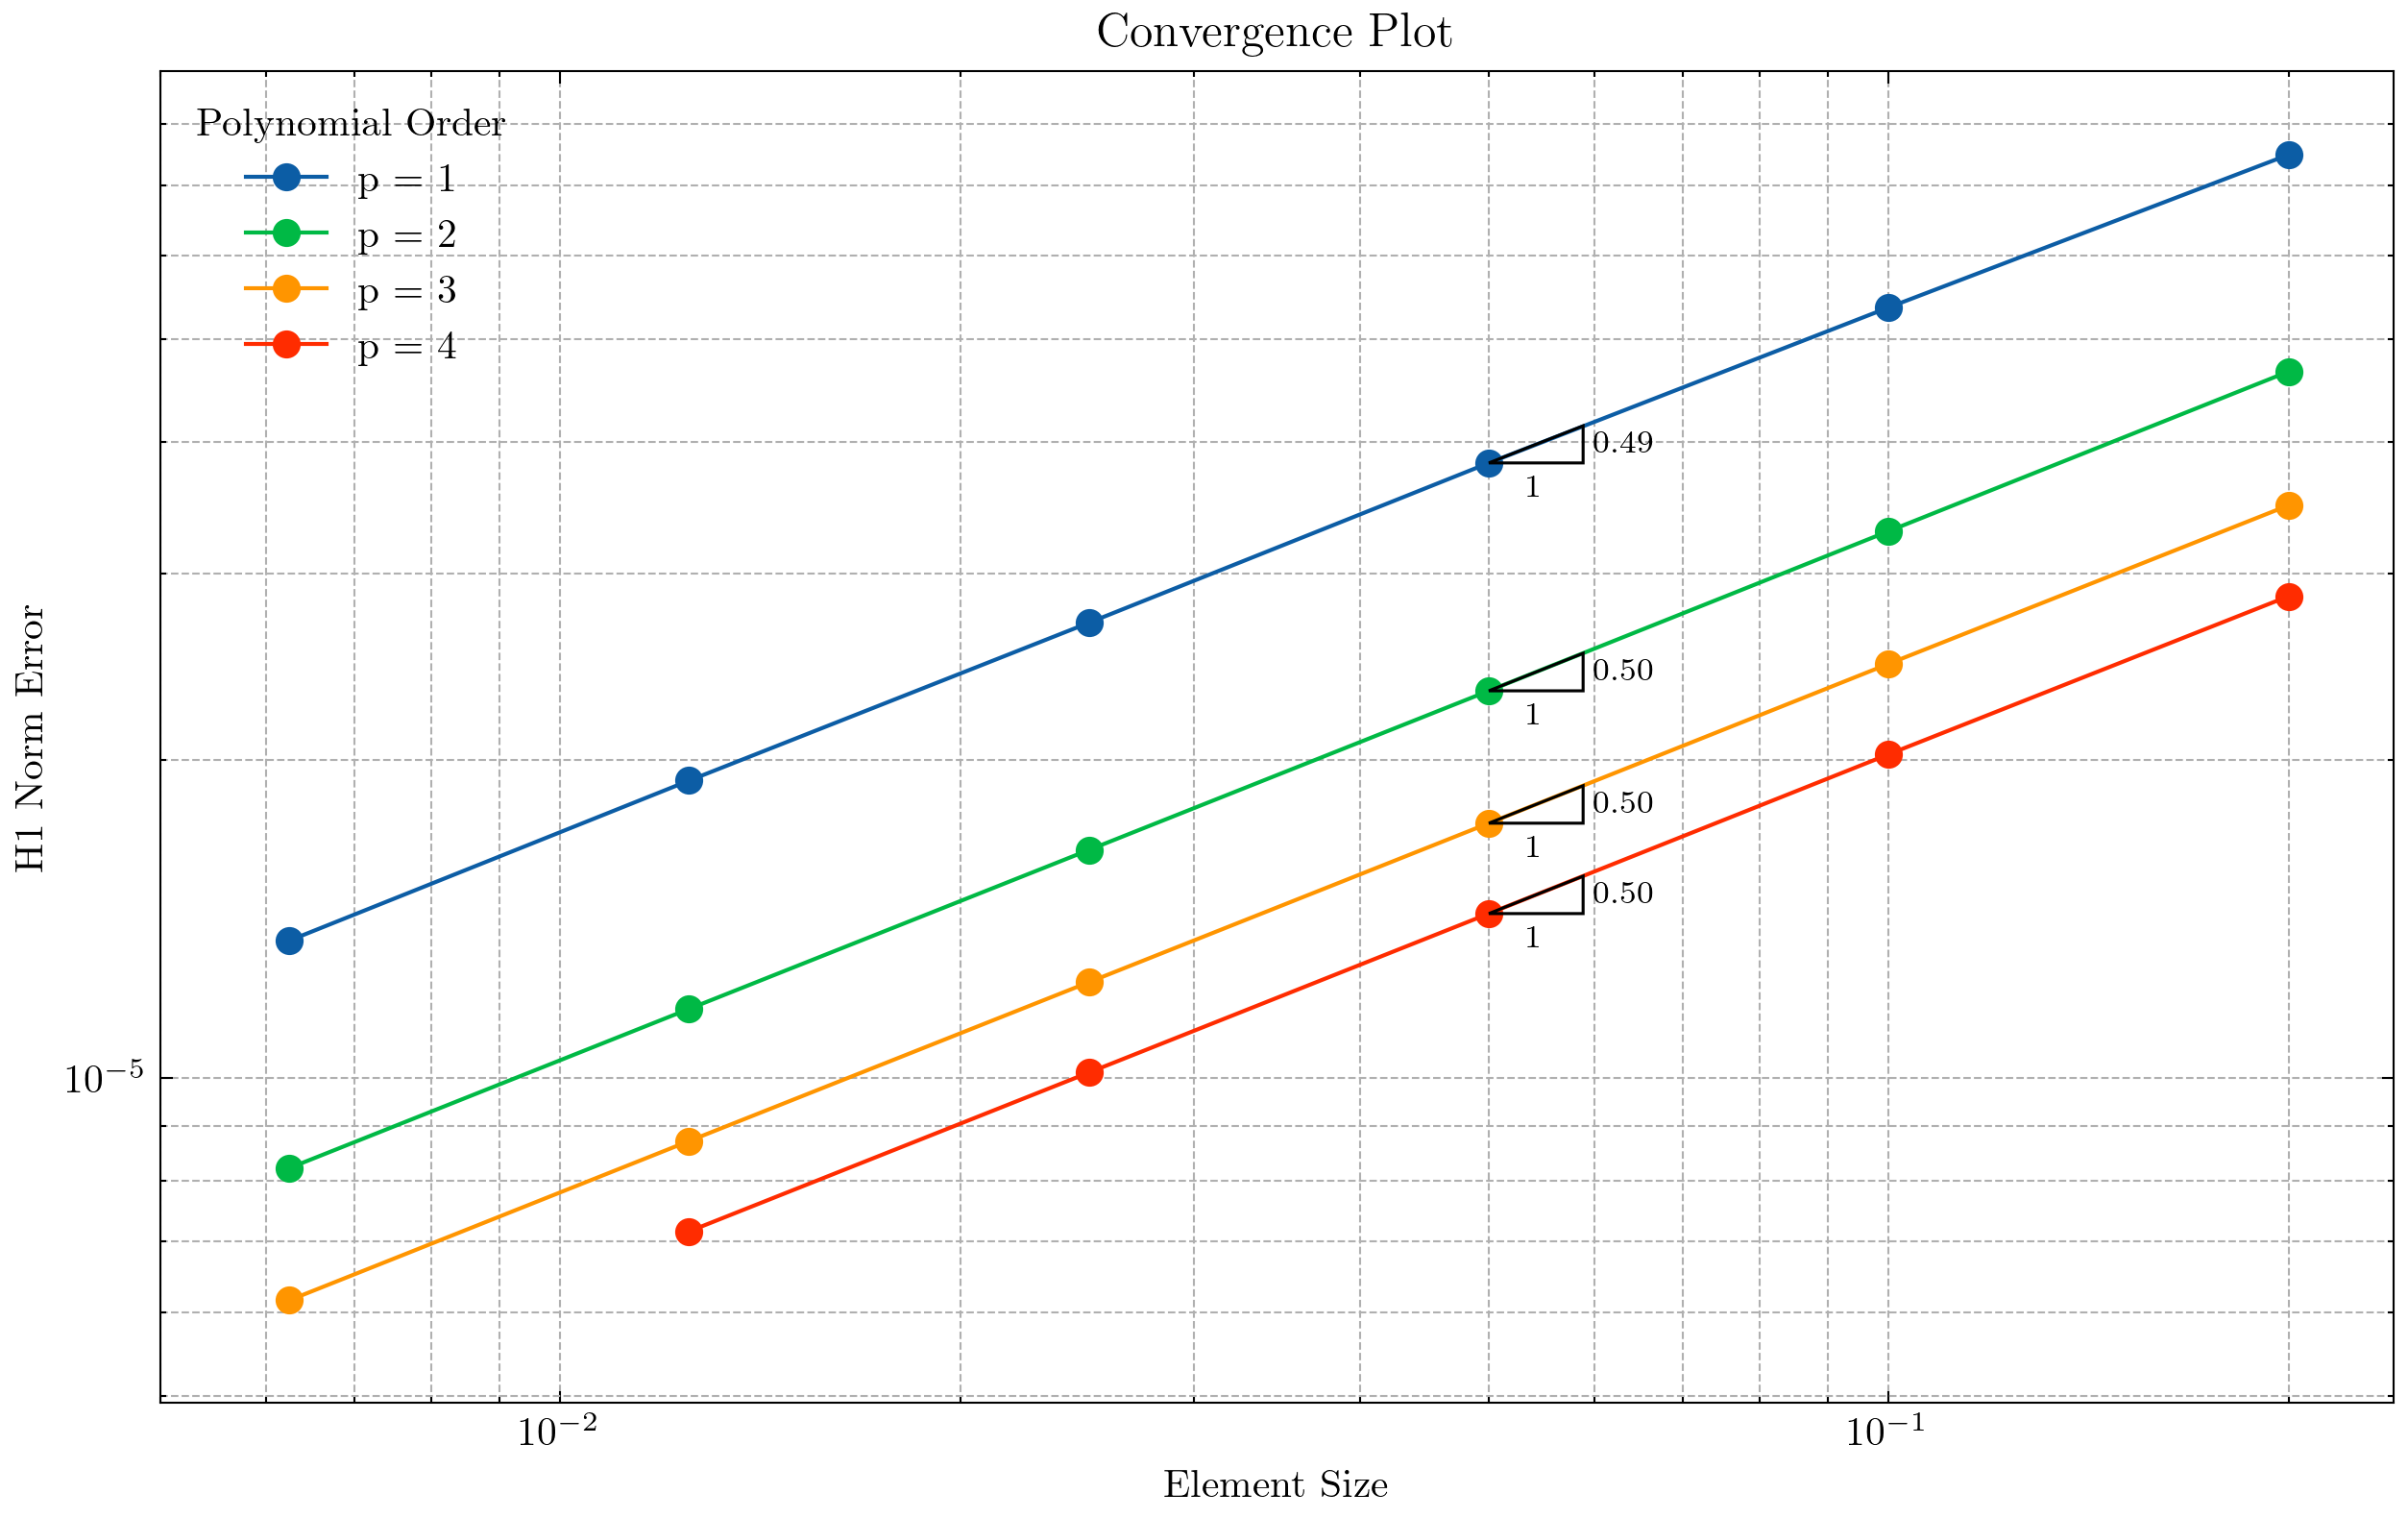
\includegraphics[width=0.5\textwidth]{Figures/convergence_plot_fem.png}\\
\scriptsize FEM convergence on crack-tip problem
\end{column}
\end{columns}
\end{frame}

% ============================================================================
\begin{frame}{Problem 2: Convergence, Iterations \& Runtime}
\begin{columns}[T]
\begin{column}{0.5\textwidth}
\centering
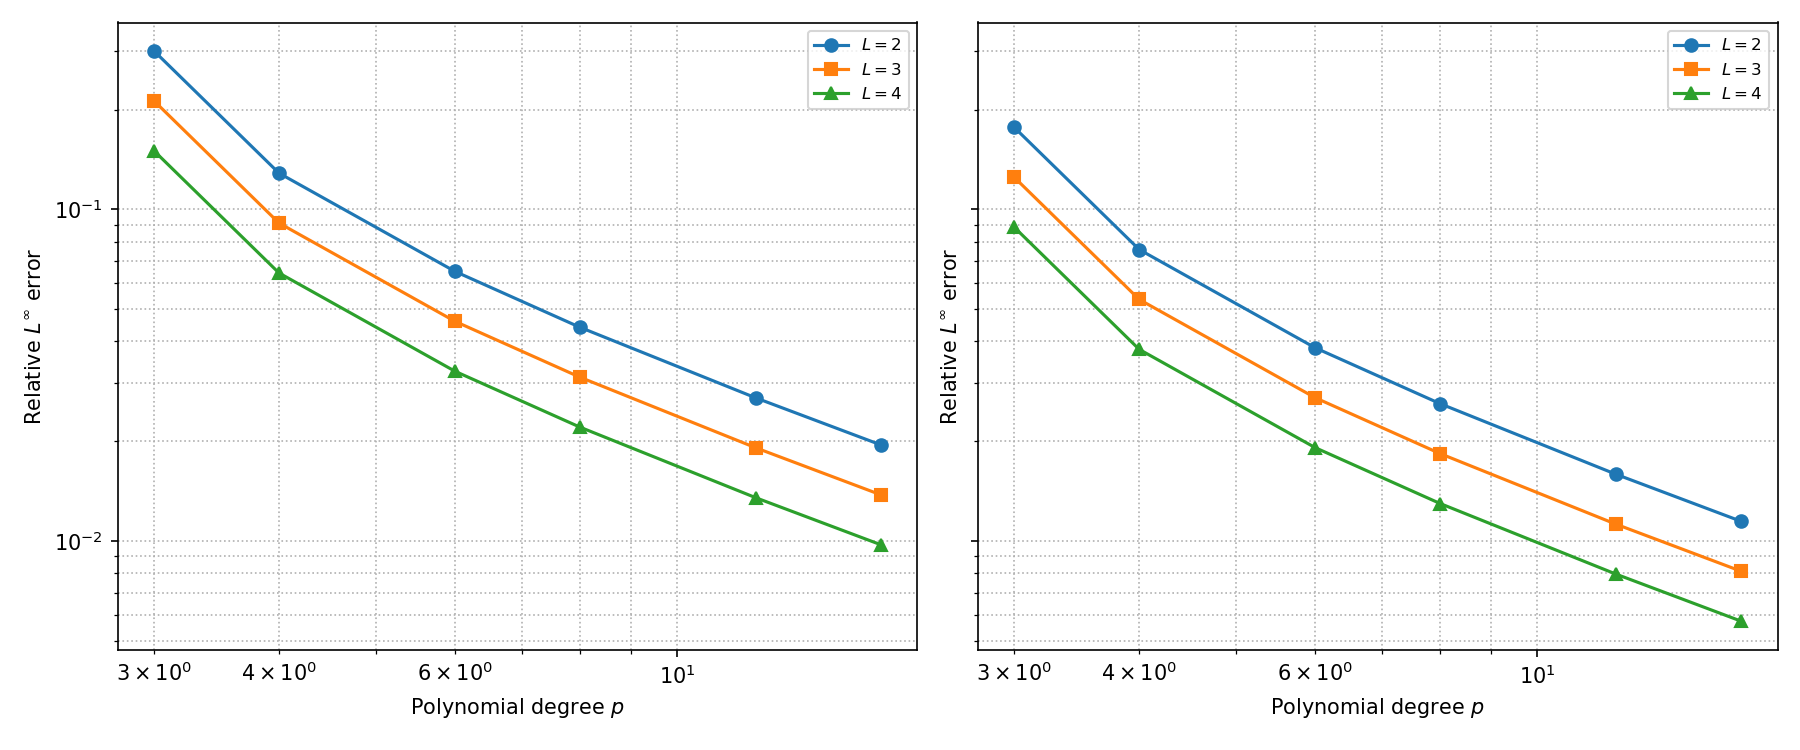
\includegraphics[width=\textwidth]{../data/examples/linear_elasticity_crack_tip_2D/error_vs_p.png}\\
\scriptsize Relative $L^\infty$ error vs.\ polynomial degree
\vspace{0.1cm}
\begin{itemize}
\scriptsize
  \item Algebraic convergence (singularity-limited)
  \item Increasing $L$ (refinement) helps
  \item Iteration count appears independent of $p$
\end{itemize}
\end{column}
\begin{column}{0.5\textwidth}
\centering
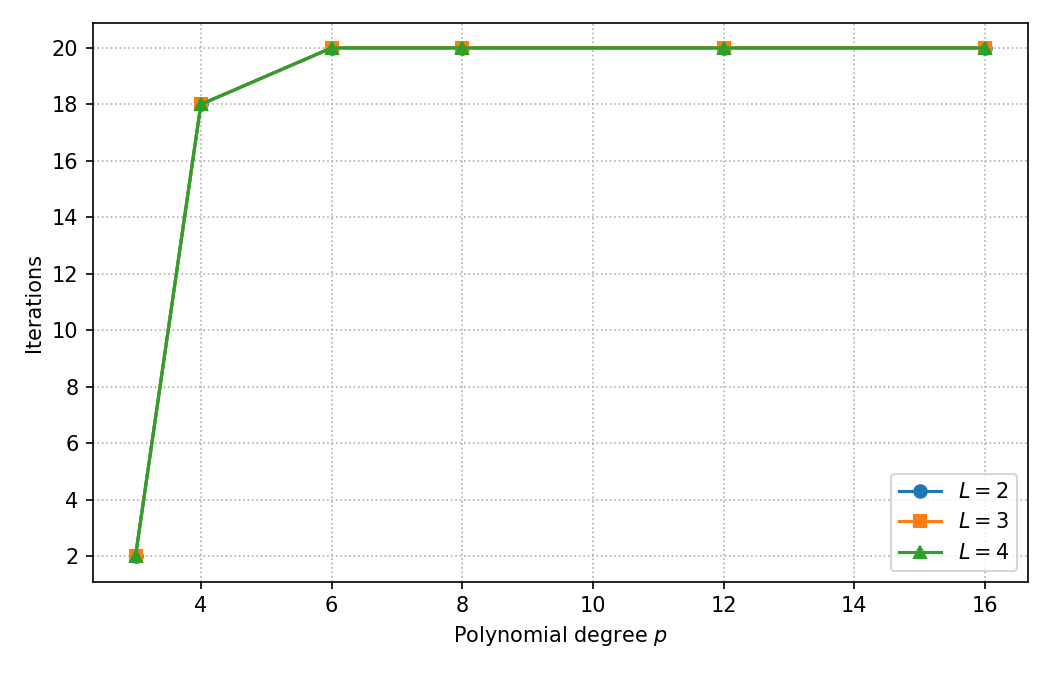
\includegraphics[width=0.7\textwidth]{../data/examples/linear_elasticity_crack_tip_2D/iterations.png}\\[0.15cm]
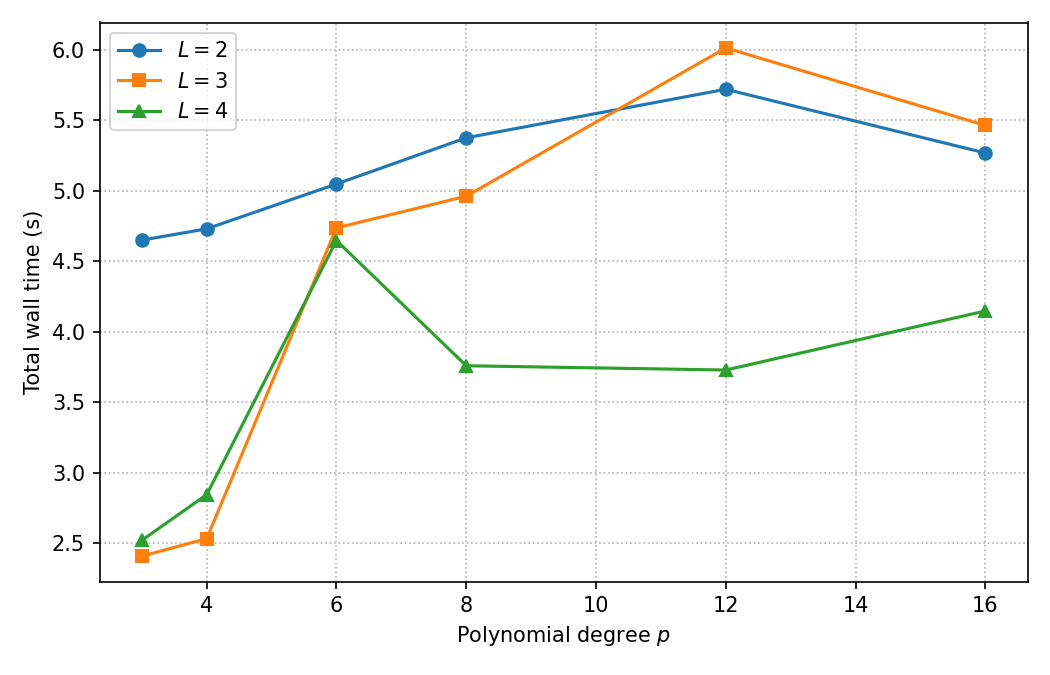
\includegraphics[width=0.7\textwidth]{../data/examples/linear_elasticity_crack_tip_2D/runtimes.png}

\end{column}
\end{columns}
\end{frame}

% ============================================================================
\begin{frame}{Problem 2: Stress Fields}
\centering
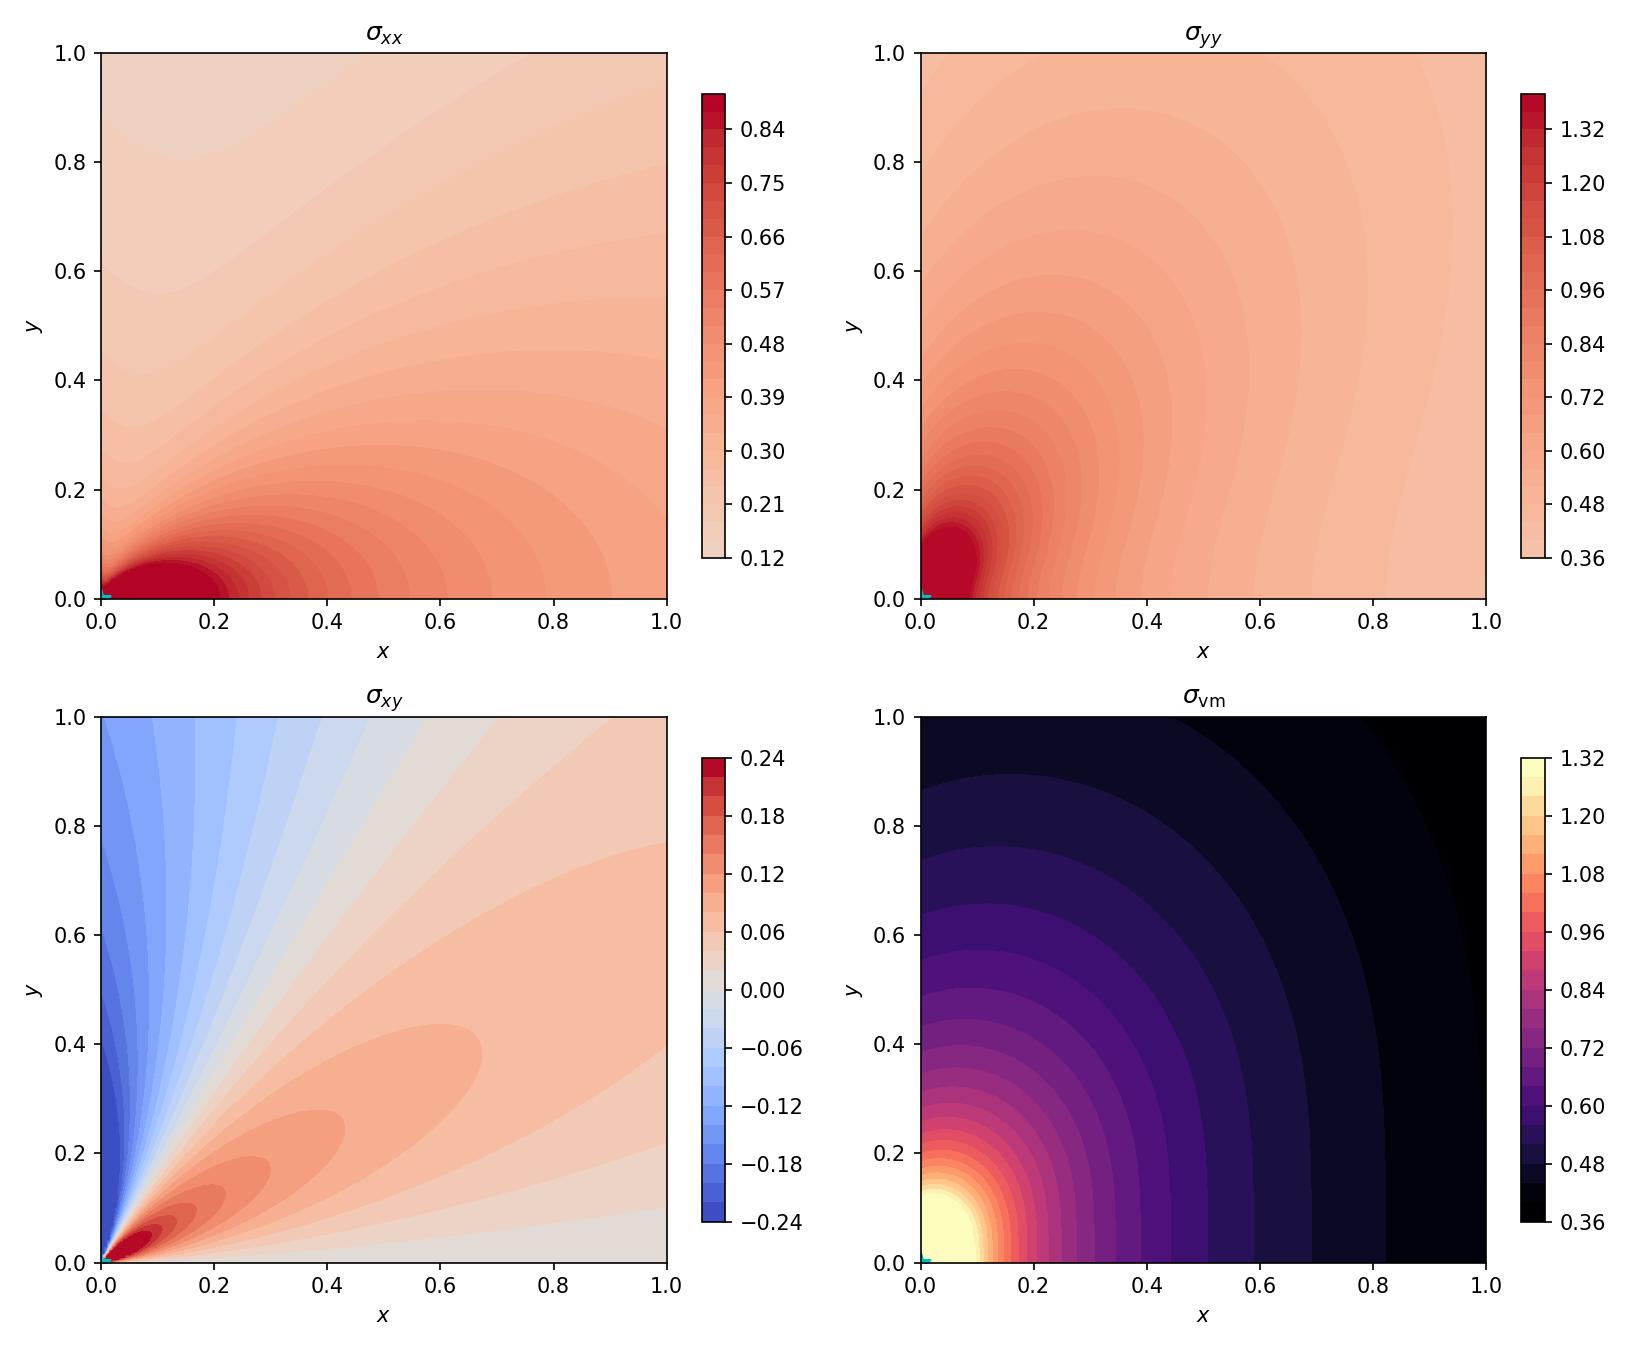
\includegraphics[height=\textheight]{../data/examples/linear_elasticity_crack_tip_2D/stress_contours.png}
\end{frame}

\section{Summary}

% ============================================================================
\begin{frame}{Conclusions}
\textbf{Main Results}
\begin{itemize}
  \item Smooth elasticity case: spectral convergence
  \item Crack-tip case: algebraic convergence due to $\frac{1}{\sqrt{r}}$ singularity
  \item ADI coupling converges seems to be independent of refinement and polynomial degree
  \item HPS remains efficient as $p$ and $L$ increase
\end{itemize}

\vspace{0.3cm}
\textbf{Next step}: Adaptive refinement near the crack tip.
\end{frame}

\end{document}
